\documentclass{szzclass}
\usepackage{hyperref}
\usepackage{longtable}
\usepackage{booktabs}

\subject{DBS}
\code{BI-SPOL-9}
\topic{Relační databáze, dotazování v relační algebře, základní koncepce jazyka SQL (SELECT, DDL, DML, DCL, TCL) , vyjádření integritních omezení v DDL.}
\providecommand{\tightlist}{%
  \setlength{\itemsep}{0pt}\setlength{\parskip}{0pt}}
\begin{document}
\tableofcontents
\newpage

\section{DBS}
DBS = database system \newline
DBMS = systém řízení bází dat (database managment system)
\begin{itemize}
  \item RDBMS = relační DBMS
  \item ODBMS = objektový DBMS
  \item ORDBMS = objektově-relační DBMS
\end{itemize}

Zabývá se seřazením velkého množství, perzistentních, spolehlivých a sdílených dat
\begin{itemize}
  \item velké množstí = pro data nestačí operační paměť
  \item perzistestní = data přetrvávají od zpracování ke zpracování
  \item spolehlivý = data lze rekonstruovat po chybě
  \item sdílených = data jsou přístupná více uživatelům
\end{itemize}
\section{Relační databáze}
(R,I) je schéma relační databáze, kde
\begin{itemize}
  \item R = {$R_1$, $R_2$, \dots, $R_n$} je množina relací
  \item I je množina integritních omezení
\end{itemize}

relace = množina n-tic $\subset D_1 \times D_2 \times \dots \times D_n$ (relace = tabulka)
\begin{itemize}
  \item jména atribubtů [$A_1, A_2, \dots, A_n$]
  \item domény atributů $D_i$
  \item v relaci nezáleží na pořadí n-tic
  \item relace neobsahuje duplicitní n-tice
\end{itemize}
\section{Relační algebra}
\begin{itemize}
  \item relační algebra je "vyšší" jazyk
  \item nespecifikujeme "jak se mají věci dělat", ale "co má být výsledkem"
  \item výsledek dorazu je relace, která může být vstupem do dalšího dotazu - jdou řetězit
  \item řeší "pouze" dotazování nikoliv DML ani DDL
\end{itemize}
\subsection{Základní operace relační algebry}
\begin{itemize}
  \item selekce (restrikce) = relace R dle podmínky $\phi$
  \begin{itemize}
    \item R($\phi$ = def\{u$|$u$\in$R $\wedge \phi (u)$\}) = množina splňující podmínku
  \end{itemize}
  \item projekce = relace R na množině atributů C, kde C $\subseteq$ A
  \begin{itemize}
    \item $R[C] = def \{u[C] | u \in R\}$ (výběr atributů)
  \end{itemize}
  \item přirozené spojení = relací R(a) a S(B) s výsledkem T(C)
  \begin{itemize}
    \item $R*S = T(A \cup B)$ (výběr n-tic = rovnosti na všech průníkových atributech A a B)
  \end{itemize}
  \item obecné spojení
  \begin{itemize}
    \item $R[t_1 \Theta t_2]S (\Theta - podminka =, >, <\dots)$ (výsledek má všechny atributy včetně duplikací)
  \end{itemize}
  \item přejmenování atributu
  \begin{itemize}
    \item t $\rightarrow$ alias
  \end{itemize}
  \item množinové opearce
  \begin{itemize}
    \item sjednocení
    \item průnik
    \item rozdíl
    \item kartézský součin
  \end{itemize}
\end{itemize}

\begin{figure}[h!]
  \centering
  
\includegraphics[width = \textwidth ]{topics/bi-spol-09/images/RaExample.png}
\end{figure}

Antijoin = podmnožina n-tic z R, které nejsou spojitelné s žádnou n-ticí z S. Minimální množinu operací
tvoří: $\times$, selekce, projekce, $\rightarrow$, $\cup$, $\backslash$.

\section{Polospojení}
Interpretace R $<$* S = podmnožina n-tic z R, které jsou spojitelné s nějakou n-ticí z S. Polospojení
není to samé jako Left/right join. Je to ověření podmínky, že mohou být spojeni.
\begin{figure}[h!]
  \centering
  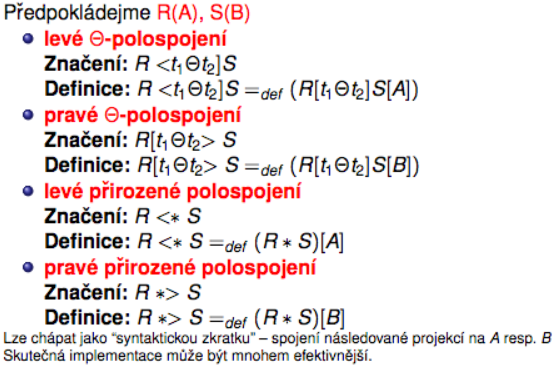
\includegraphics[width = \textwidth ]{topics/bi-spol-09/images/halfConnection.png}
\end{figure}
Relační dělení:
Interpretace $R \div S$ = výsledkem jsou všechny hodnoty x z R, které v R tvoří dvojici s každým prvkem y z S.
Pomocí prvků y z S se snažíme diskvalifikovat prvky x z R. Prvek x je diskvalifikován, pokud v R neexistuje ve dvojici s každým y z S.
Výsledkem R $\div$ S jsou prvky x z R, které se diskvalifikovat nepodařilo.
\begin{itemize}
  \item R(x, y) a S(y)
  \item značení = R $\div$ S
  \item definice = $R \div S =_{def} R[x] \backslash \{\{R[x] \times S\} \backslash R\}[x]$
\end{itemize}

\begin{figure}[h!]
  \centering
  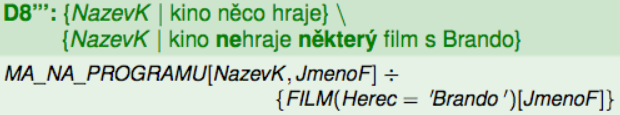
\includegraphics[width = \textwidth ]{topics/bi-spol-09/images/division.png}
\end{figure}

\section{SQL}
\begin{itemize}
  \item SQL = (Structured query language) 
  \item slouží ke komunikaci s databázovým strojem
  \item říkáme, co chceme získat, ne jak se to má dělat
  \item intuitivně srozumitelný zápis
  \item připomíná jednoduché anglické věty
\end{itemize}

\begin{description}
  \item[DDL] Definiční jazyk -- např. manipulace s tabulkama, integritní omezení \texttt{CREATE TABLE}
  \item[DML] Manipulační jazyk -- např. \texttt{SELECT, INSERT, UPDATE} apod.
  \item[DCL] Jazyk na přístupy -- \texttt{GRANT <prikaz> ON <table> TO <user>}
  \item[TCL] Jazyk pro řízení transakcí -- \texttt{COMMIT}, \texttt{ROLLBACK}
\end{description}

\begin{verbatim}
SELECT sloupce
FROM tabulky
[WHERE podmínky]
[ORDER BY řazení]
\end{verbatim}

\section{Integritní omezení}
Omezení domény (tabulek)
\begin{itemize}
  \item NOT NULL
  \item DEFAULT
  \item UNIQUE
  \item PRIMARY KEY
  \item REFERENCES
  \item CHECK
\end{itemize}

Okamžik kontroly IO, dočasné vypnutí/zapnutí IO:
\begin{itemize}
  \item možnosti stanovit při deklaraci integritního omezení čas, kdy se má kontrolovat
  \item kontrolu IO lze definovat jako odložitelnou až na konec transakce
  \item v rámci session pak lze stanovit, zda IO kontruje IMMEDIATE nebo až na konci transakce
  \item Oracle dovoluje v příkazu ALTER TABLE také IO dočasně vypnout/zneplatnit DISABLE/ENABLE CONSTRAINT
  \item zpětně zapnutí IO pak může/nemusí vyžadovat kontrolu platnosti dat již vložených v databázi
\end{itemize}
% \section{Dotazování v relační algebře}
% \begin{itemize}
%   \item Relační algebra je pouze dotazovací formalismus. (Pokrývá jenom \mintinline{sql}{SELECT} v SQL.)
%   \item 
% \end{itemize}
% \section{Základní koncepce jazyka SQL (\mintinline{sql}{SELECT}, DDL, DML, DCL, TCL)}
% \begin{description}
%   \item[DDL] Definiční jazyk -- např. manipulace s tabulkama, integritní omezení
%   \item[DML] Manipulační jazyk -- např. \mintinline{sql}{SELECT}, \mintinline{sql}{INSERT}, \mintinline{sql}{UPDATE} apod.
%   \item[DCL] Jazyk na přístupy
%   \item[TCL] Jazyk pro řízení transakcí
% \end{description}



% \section{Vyjádření integritních omezení v DDL}

\end{document}
